\documentclass[12pt]{article}

\usepackage[spanish]{babel}
\usepackage[utf8]{inputenc}
\usepackage{graphicx}
\usepackage{geometry}
\usepackage{xcolor}
\usepackage{fancyhdr}
\usepackage{lastpage}
\usepackage{pdfpages}
\usepackage{listings}

\geometry{top=25mm,left=15mm,right=15mm,a4paper}

\pagestyle{fancy}
\fancyhf{}
\lhead{Sistemas Operativos}
\cfoot{Página \thepage\ de \pageref{LastPage}}

\graphicspath{./}

\begin{document}
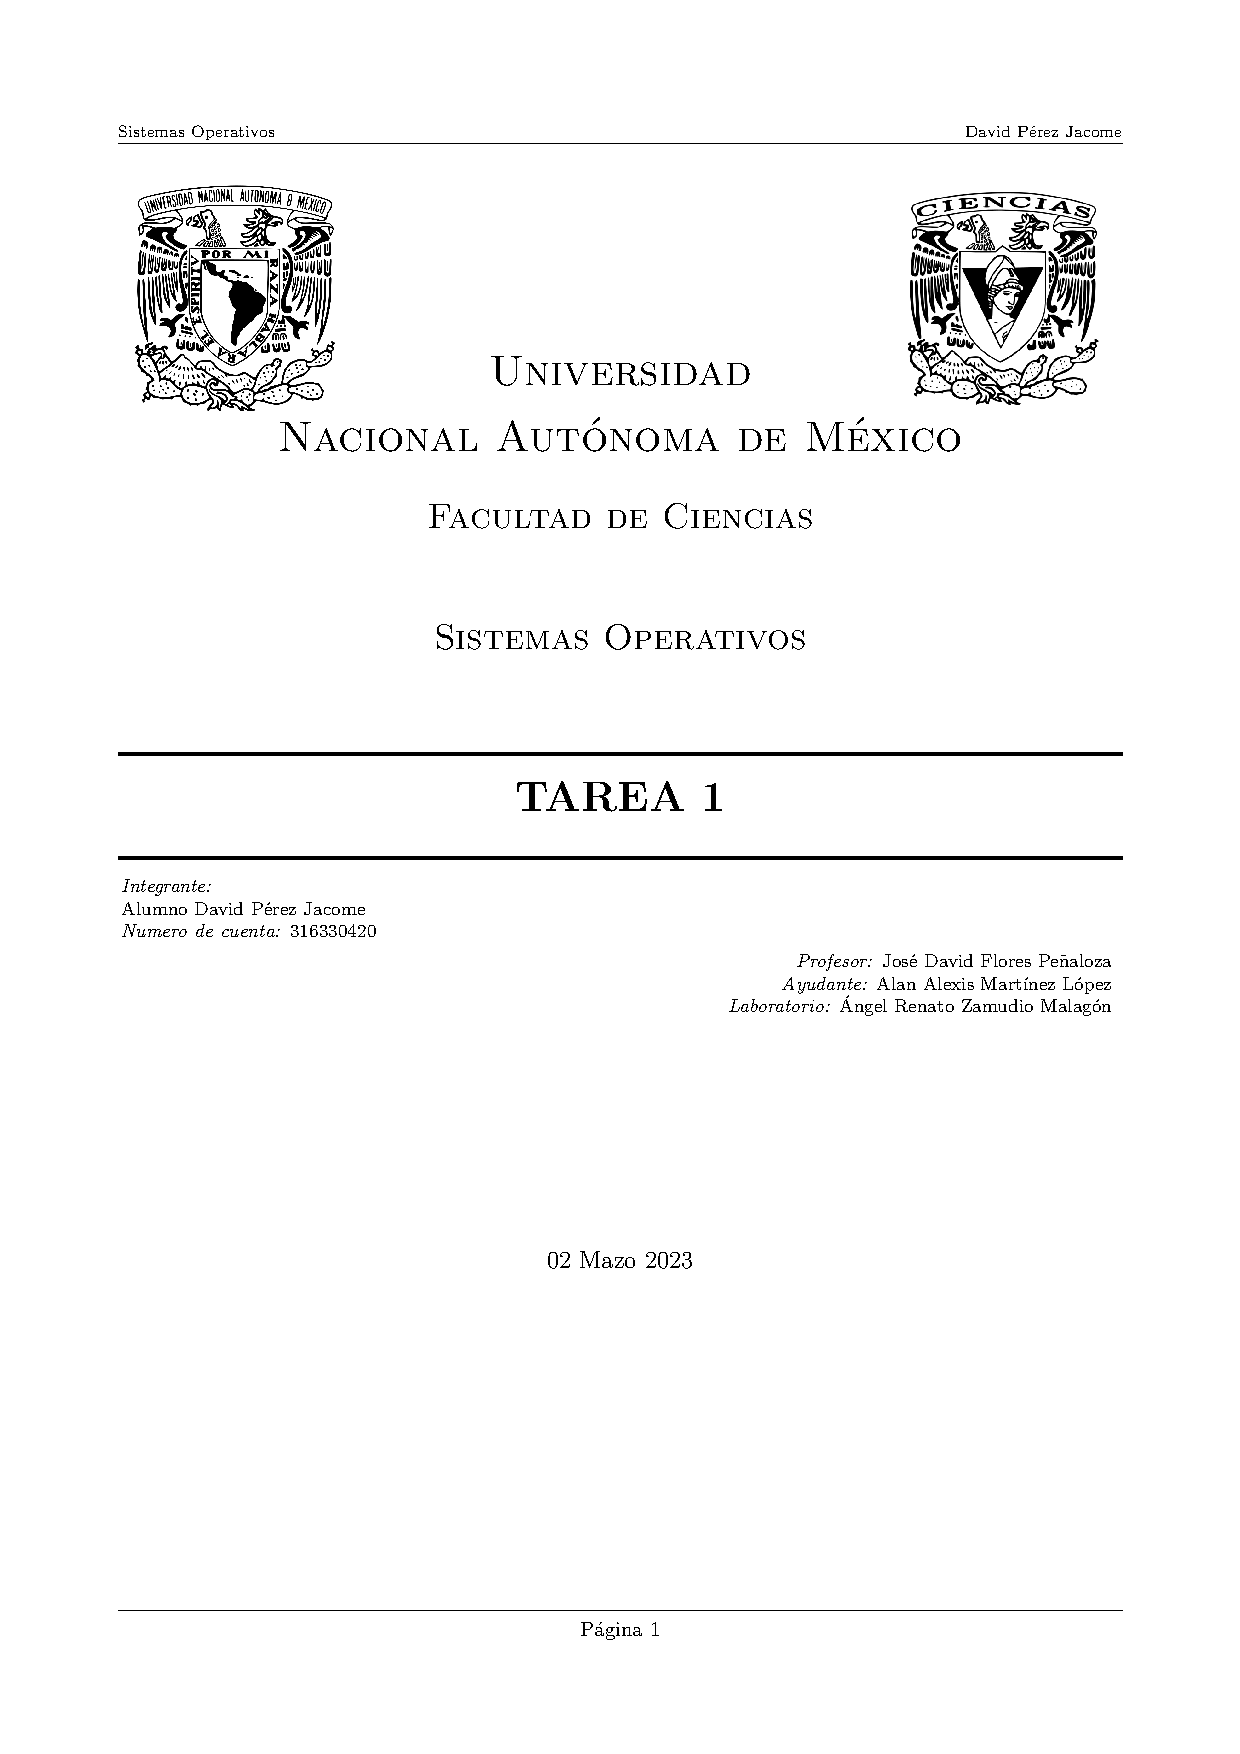
\includepdf{Portada.pdf}
{\color{blue} \section*{Tarea 1.}}

{\color{blue} \subsection*{Instrucciones.}}
\vspace{0.5em} 

Lee con atención las preguntas y contesta lo correspondiente. La tarea se entregará por vía classroom
en un archivo pdf que debe tener el nombre completo y número de tarea, ya sea en una portada o en el encabezado.
\textbf{La tarea se entregará de manera individual.}\\

{\color{blue} \subsection*{Ejercicios}}
\vspace{0.5em}

\begin{enumerate}
    \item Describe brevemente y con tus palabras. ¿Qué es un Sistema Opertivo?
    \item ¿Cuáles son las principales tareas de un sistema operativo?
    \item ¿Cúales son los pasos a seguir que siempre debe hacer un \textbf{CPU} (microprocesador)? Explicalas brevemente.
    \item Describe las caracteristicas principales de la memoria primaria. Y menciona un ejemplo.
    \item Describe las caracteristicas principales de la memoria secundaria. Y menciona un ejemplo.
    \item ¿Por qué se cambio la arquitectura de un sistema de computo de un solo procesador a multiprocesadores?
    \item ¿Por qué los sistemas de computo son orientados a interrupciones?
    \item ¿Qué es una interrupción de software y para qué se utilizan?
    \item ¿Qué es un controlador de dispositivo? 
\end{enumerate}

\end{document}